\documentclass[11pt,letterpaper]{article}
\usepackage[top=2.0cm, bottom=3cm, left=2.0cm, right=2.0cm]{geometry}
\usepackage[utf8]{inputenc}
\usepackage[T1]{fontenc}
\usepackage[spanish]{varioref}
\usepackage[activeacute, spanish, es-tabla]{babel}
\usepackage{fancyhdr}
\usepackage{multicol}
\usepackage{float}
\usepackage{textcomp}
\usepackage{ae,aecompl}
\usepackage{amssymb,amsmath}
\usepackage[pdftex]{graphicx}
\pagestyle{fancy} 
\pagenumbering{arabic} 
\renewcommand{\headrulewidth}{0pt} 
\setlength{\headsep}{20pt} 
\setlength{\headheight}{65pt} 
\setlength{\textheight}{600pt} 
\setlength{\columnsep}{15pt} 
\newcommand{\universidad}{\small{Universidad Técnica Federico Santa María}}
\newcommand{\campus}{\small{Campus Santiago San Joaquín}}
\newcommand{\semestre}{\small{Segundo Semestre 2016}}

% Definiciones de Título e Integrantes de Experiencia
\newcommand{\titulo}{Tarea 4 - TALF}
\newcommand{\integrantes}{\begin{tabular}{c}
Jorge Contreras 201573547-6 \\
Juan Pablo Jorquera  201573533-6 \\
\end{tabular}}

\renewcommand{\maketitle}
{
\thispagestyle{fancy}
\begin{center}
\begin{Large}
\textbf{\titulo}\\
\end{Large}
\vspace{0.5cm}
\integrantes
\end{center}
\vspace{0.3cm}
}


%ENCABEZADO

\fancyhead[R]{\begin{minipage}[b]{0.405\textwidth}
\begin{center}
\universidad \\ 
\campus \\ 
\lab \\ 
\semestre
\end{center}
\end{minipage}}
\fancyhead[L]{\vspace{15pt}
\includegraphics[height=1.6cm]{Escudo.png}}
%%%%%%%%%%%%%%%%%%%%%%%%%%%%%%%%%%%%%%%%%%%%%%%%
%                                              %
% AQUI TERMINAN LAS DEFINICIONES DE ENCABEZADO %
% Y EMPIEZA EL CUERPO DEL DOCUMENTO            %
%                                              %
%%%%%%%%%%%%%%%%%%%%%%%%%%%%%%%%%%%%%%%%%%%%%%%%

\begin{document}
\maketitle

\section{Pregunta 1}
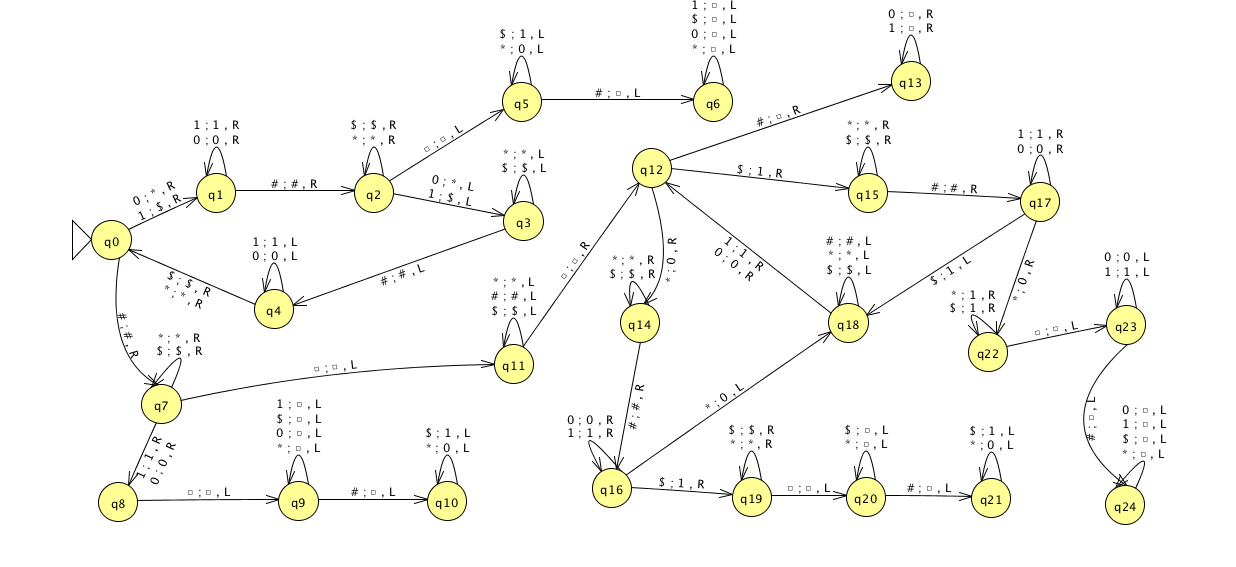
\includegraphics[height=8cm]{p1.png}
La máquina de Turing se divide en dos grandes partes: inicialmente compara los tamaños para decidir cual es el menor y luego, de ser iguales compara término a término para definir el menor.
\begin{itemize}
	\item Entre q0 y q4 va marcando los 1 con \$ y los 0 con * y luego verifica que exista ese dígito en el término de la derecha.
	\item En q2 se sale al haber encontrado un dígito a la izquierda y haber terminado por completo el de la derecha, entonces el de la derecha es más corto, y en q5 y q6 lo decodifica y limpia el resto.
	\item En q0 se sale al haber terminado el primer término, entonces avanza hasta la posición actual del término de la derecha y verifica si también terminó.
	\item En caso de no haber terminado significa que el término de la izquierda era menor, entonces en q8, q9 y q10, limpia el término de la derecha y decodifica el de la izquierda.
	\item Por otro lado si también termina el término de la derecha, significa que eran de igual tamaño, donde avanza a q11 y de aquí se devuelve al comienzo de la cinta.
	\item Acá para comparar son dos partes virtualmente simétricas, dependiendo si comienza con 0 o 1 (codificado), lo decodifica y avanza al término de la derecha para comparar hasta q16 y q17 respectivamente.
	\item En caso de encontrar el mismo valor, se devuelve a q12 para seguir comparando.
	\item De no ser así se sale en q19 y q22 para terminar devolviendo el término adecuado en el resto de los nodos de esta rama.
	\item Finalmente en la situación de que ambos sean completamente iguales, se sale de q12 a q13, estándo ya decodificados por el loop los términos, simplemente borra el de la derecha.
\end{itemize}

\section{Pregunta 2}
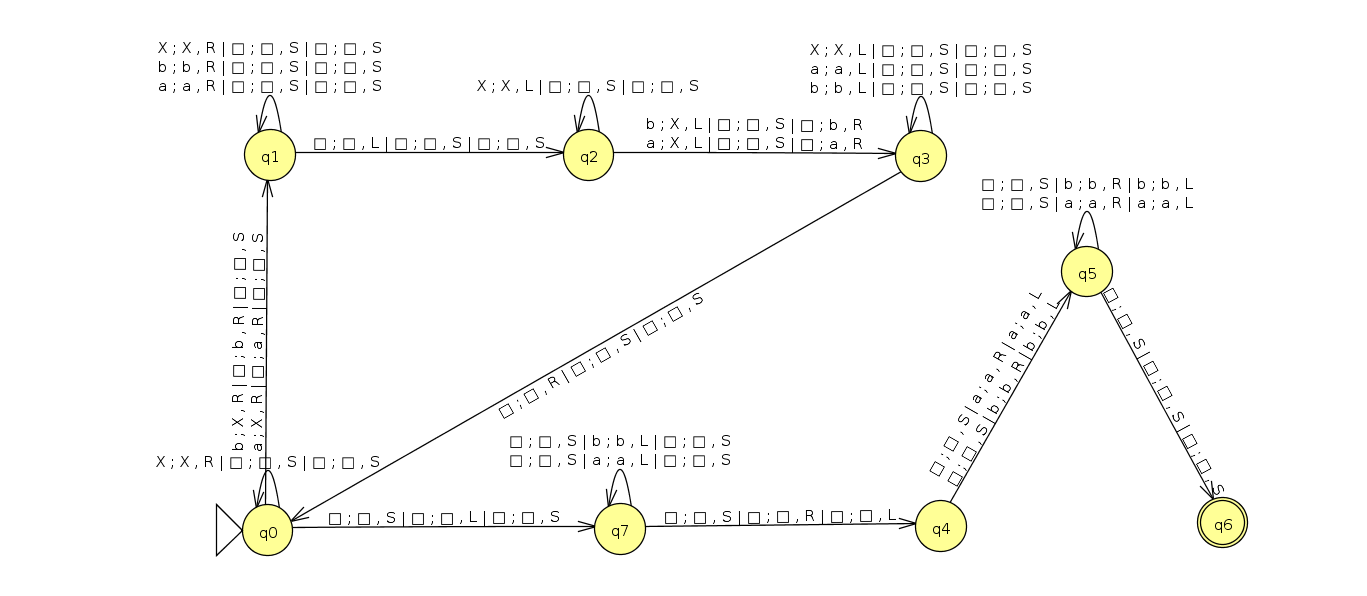
\includegraphics[height=8cm]{p2.png}
La maquina de Turing presenta tres cintas, la primera es aquella que presenta el input w y las otras dos son cintas inicialmente vacías. \\
El funcionamiento de la maquina es sencillo, y al igual que el anterior se divide en dos partes:
\begin{itemize}
	\item El loop presente en la maquina (q0, q1, q2, q3) refiere a leer la primera palabra de w y escribirla en la segunda cinta, dejándola como $"X"$ en la primera, luego se dirige al final de la primera cinta y lee el último termino para escribirlo en la tercera cinta dejando el valor de la primera como $"X"$ nuevamente. Realiza el mismo proceso con la segunda y penúltima letra y así sucesivamente. Si la cantidad de letras es impar no logra entrar a la segunda parte, en cambio si la cantidad es par sí entra.
	\item Cuando la cantidad de letras es par entra en esta sección (q7), lo primero que hace es llevar la segunda cinta al inicio para luego empezar a comparar la segunda y tercera cinta, como la tercera cinta se empezó escribiendo de atrás para adelante se compara la segunda cinta desde el inicio moviéndose hacia la derecha y la tercera desde el final moviéndose a la izquierda, si la comparación es fructífera llega al estado de aceptación, si no lo es, no lo hará.
\end{itemize}

\section{Pregunta 3}
Vamos a demostrar que hay equivalencia entre las MT comunes y las que incluyen las trancisiones creadas por Juan Turing Contreras, sólo bastaría en lugar de pasar el input requerido para la transición, utilizar el complemento de él, donde por letra se realiza la misma transición, lo que podemos ver fácilmente en el ejemplo entregado:
Con L = \{a,b,c\}.
\begin{center}
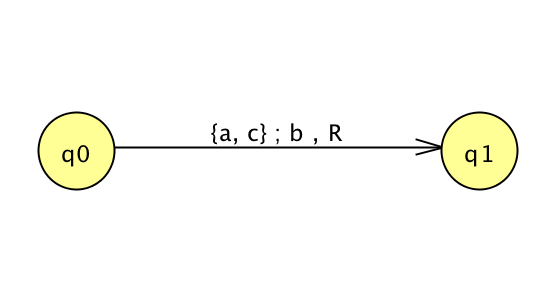
\includegraphics[height=4.2cm]{p3a.png}
\end{center}
Donde la transición simplemente pasaría a ser el complemento del input \{a,c\} en MT:
\begin{center}
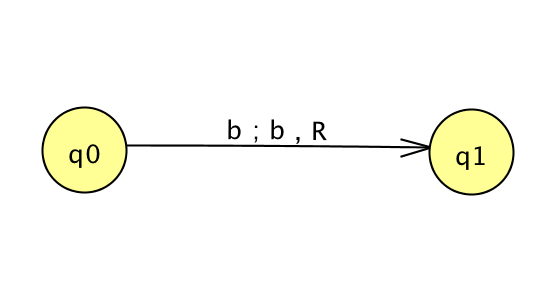
\includegraphics[height=4.2cm]{p3b.png}
\end{center}
Acá también es fácil ver que nuevamente para hacer el camino hacia el otro lado es de igual forma, utilizando el complemento de \{b\}, por lo que notamos que ésto se puede realizar para cualquier transición que haya, por lo que generalizando lo antes dicho:

Siendo $L_1$ el conjunto de letras que se incluyen en la transición de la nueva MT, su transición correspondiente sería $\delta(q_x, L_1) = (q_y, v, Mov)$, donde $v$ es por lo que se quiere reemplazar y $Mov$ el lado hacia el que se quiere mover, entonces en MT comunes correpondería al conjunto de trancisiones de la forma $\delta(q_x, u) = (q_y, v, Mov), \forall u \in L_1^c$. 

Por otro lado si se tiene una trancision de una MT común $\delta(q_x, u) = (q_y, v, Mov), u \in L_2$ se traduce a la nueva MT como $\delta(q_x, L_2 - \{u\}) = (q_y, v, Mov)$, por lo que queda entonces demostrado.


\section{Pregunta 4}
\subsection{Parte a}
Tenemos dos casos que analizar, en primer lugar que sucede si usa su segunda cinta, entonces simplemente nuestra máquina se detiene; por otro lado, si no hace uso de la segunda cinta se queda pegada en un loop intentando hasta que se haga uso de ella.
Por lo que este problema sería equivalente a resolver el problema del alto, el cual sabemos que es indecidible, por lo que de igual forma es indecidible.

\subsection{Parte b}
Para determinar si existe o no una infinidad de distintos inputs entregados a dos maquinas de Turing, hay que primero determinar si existe o no una cantidad finita de inputs que las maquinas acepten, por lo tanto podemos reducir este problema a un problema de membresía, dado que si es indecidible poder comprobar que un input en particular es aceptado por una maquina, es indecidible también determinar si infinitos inputs son aceptados por una maquina, aún menos si estos son aceptados por dos maquinas a la vez, concluyendo así que se trata de un problema indecidible.

\end{document}
